\documentclass[aspectratio=169]{beamer}
\usepackage{will_handley}

% Commands
% --------
% - \arxiv{arxiv number}
% - \cols{width}{lh column}{rh column}
% -  \begin{fig(left|right)}[fractional width (e.g 0.6) ]{name of image}
%        content of other column
%    \end{fig(left|right)}

% Talk details
% ------------
\title{Nested Sampling and Likelihood Free Inference}
\date{21\textsuperscript{st} April 2022}
%Nested Sampling is an established numerical technique for optimising,
%sampling, integrating and scanning *a priori* unknown probability
%distributions. Whilst typically used in the context of traditional
%likelihood-driven Bayesian inference, it's capacity as a general sampler means
%that it is capable of exploring distributions on data [2105.13923] and joint
%spaces [1606.03757].  
%
%In this talk I will give a brief outline of the points
%of difference of nested sampling in comparison with other techniques, what it
%can uniquely offer in tackling the challenge of likelihood-free inference, and
%discuss ongoing work with collaborators in applying it in a variety of
%LFI-based approaches.

\begin{document}

\begin{frame}
    \titlepage
\end{frame}

\begin{frame}
    \frametitle{<+Frame title+>}
    <+Content+>
\end{frame}


\begin{frame}
    \frametitle{What is Nested Sampling?}
    \begin{itemize}
        \item Nested sampling is a multi-purpose numerical mathematical tool.
        \item Given a (scalar) function $f$ with a vector of parameters $\theta$, it can be used for:
    \end{itemize}
    \vspace{-10pt}
    \begin{columns}[t]
        \column{0.33\textwidth}
        \begin{block}{Optimisation}
            \vspace{-5pt}
            \[\theta_\mathrm{max} = \max_\theta{f(\theta)}\]
        \end{block}
        \column{0.33\textwidth}
        \begin{block}{Sampling}
            \vspace{-5pt}
            \[\text{draw }\theta\sim f\]
        \end{block}
        \column{0.33\textwidth}
        \begin{block}{Integration}
            \vspace{-5pt}
            \[\int f(\theta) dV \]
            \vspace{-15pt}
        \end{block}
    \end{columns}
    \begin{columns}[t]
        \column{0.33\textwidth}
            \centerline{\includegraphics[width=0.8\textwidth,page=13]{figures/himmelblau}}
        \column{0.33\textwidth}
            \centerline{\includegraphics[width=0.8\textwidth,page=15]{figures/himmelblau}}
        \column{0.33\textwidth}
            \centerline{\includegraphics[width=0.8\textwidth,page=14]{figures/himmelblau}}
    \end{columns}
\end{frame}

\begin{frame}
    \frametitle{MCMC sampling}
    Unnormalised posteriors

    Cannot compute the normalising constant
\end{frame}

\begin{frame}
    \frametitle{Nested sampling}
    \cols[0.6]{
  \begin{itemize}
    \item Nested sampling is a completely different way of sampling. 
    \item Uses ensemble sampling to compress prior to posterior.
      \item Maintain a set $S$ of $n$ samples, which are sequentially updated:
  \begin{description}
      
    \item[$S_0$:] Generate $n$ samples uniformly over the space (from the prior $\pi$). 
      
    \item[$S_{n+1}$:] Delete the lowest likelihood sample in $S_{n}$, and replace it with a new uniform sample with higher likelihood
  \end{description}
 \item Requires one to be able to sample uniformly within a region, subject to a {\em hard likelihood constraint}.
  \end{itemize}
    }{
        \includegraphics<1|handout:0>[width=\textwidth,page=1]{figures/himmelblau}
        \includegraphics<2|handout:0>[width=\textwidth,page=2]{figures/himmelblau}
        \includegraphics<3|handout:0>[width=\textwidth,page=3]{figures/himmelblau}
        \includegraphics<4          >[width=\textwidth,page=4]{figures/himmelblau}
        \includegraphics<5|handout:0>[width=\textwidth,page=5]{figures/himmelblau}
        \includegraphics<6|handout:0>[width=\textwidth,page=6]{figures/himmelblau}
        \includegraphics<7|handout:0>[width=\textwidth,page=7]{figures/himmelblau}
        \includegraphics<8|handout:0>[width=\textwidth,page=8]{figures/himmelblau}
        \includegraphics<9|handout:0>[width=\textwidth,page=14]{figures/himmelblau}
    }
\end{frame}

\begin{frame}
    \frametitle{Nested sampling}
    \cols[0.6]{
  \begin{itemize}
      \item At the end, one is left with a set of discarded points
      \item These may be weighted to form weighted posterior samples using $w_i = \mathcal{L}_i \Delta X_i$
      \item They can also be used to calculate the normalising constant $\mathcal{Z} = \sum \mathcal{L}_i \Delta X_i$.
          \begin{itemize}
              \item Nested sampling probabilistically estimates the volume of the parameter space
                  \[X_i \approx {\left(\frac{n}{n+1}\right)} X_{i-1} \quad\Rightarrow\quad
                  X_i \approx {\left(\frac{n}{n+1}\right)}^i \approx e^{-i/n} \]
              \item only statistical estimates, but we know the error bar
              \item Nested sampling thus estimates the density of states
              \item it is therefore a partition function calculator
          \end{itemize}
      \item The evolving ensemble of live points allows algorithms to perform self-tuning and mode clustering.
  \end{itemize}

    }{
        \includegraphics<1|handout:0>[width=\textwidth,page=14]{figures/himmelblau}
        \includegraphics<2          >[width=\textwidth,page=15]{figures/himmelblau}
    }

\end{frame}

\begin{frame}
    \frametitle{Implementations of Nested Sampling}
    %\begin{columns}
    %    \begin{column}{0.33}
    %        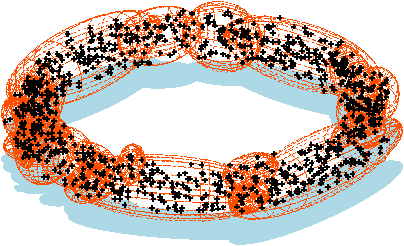
\includegraphics[width=\textwidth]{figures/multinest}
    %    \end{column} 
    %\end{columns}
    \cols[0.5]{%
        \texttt{MultiNest}
        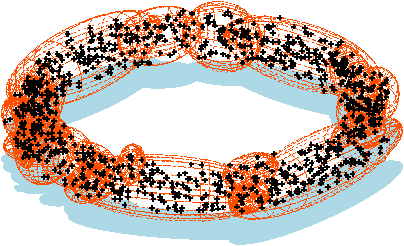
\includegraphics[width=0.8\textwidth]{figures/multinest}
            \vfill
        \texttt{DNest}
        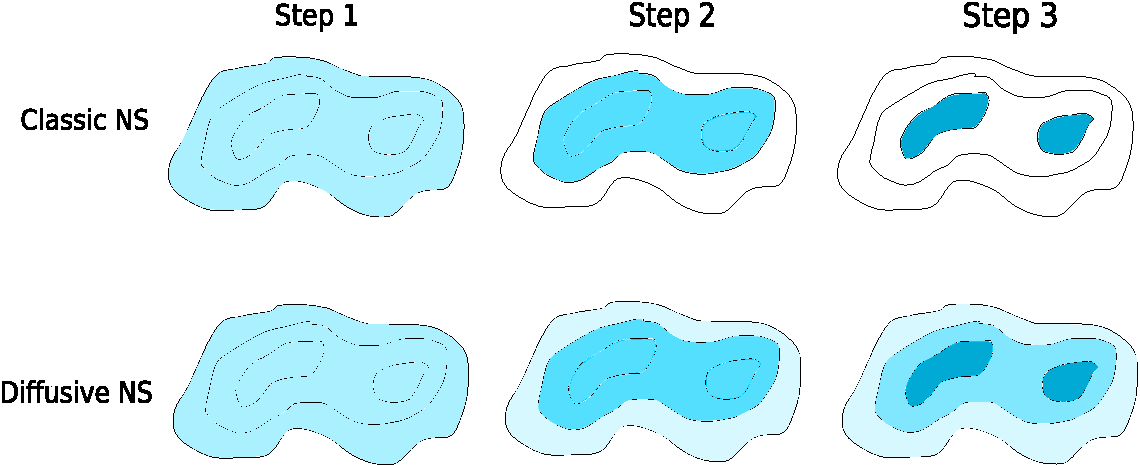
\includegraphics[width=\textwidth]{figures/dnest}
    }{%
        \texttt{PolyChord}
        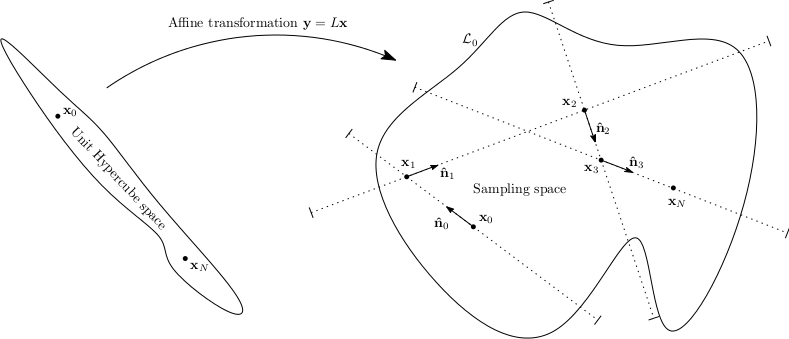
\includegraphics[width=\textwidth]{figures/polychord}
        \vfill
        \texttt{NeuralNest}
            \cols[0.5]{
                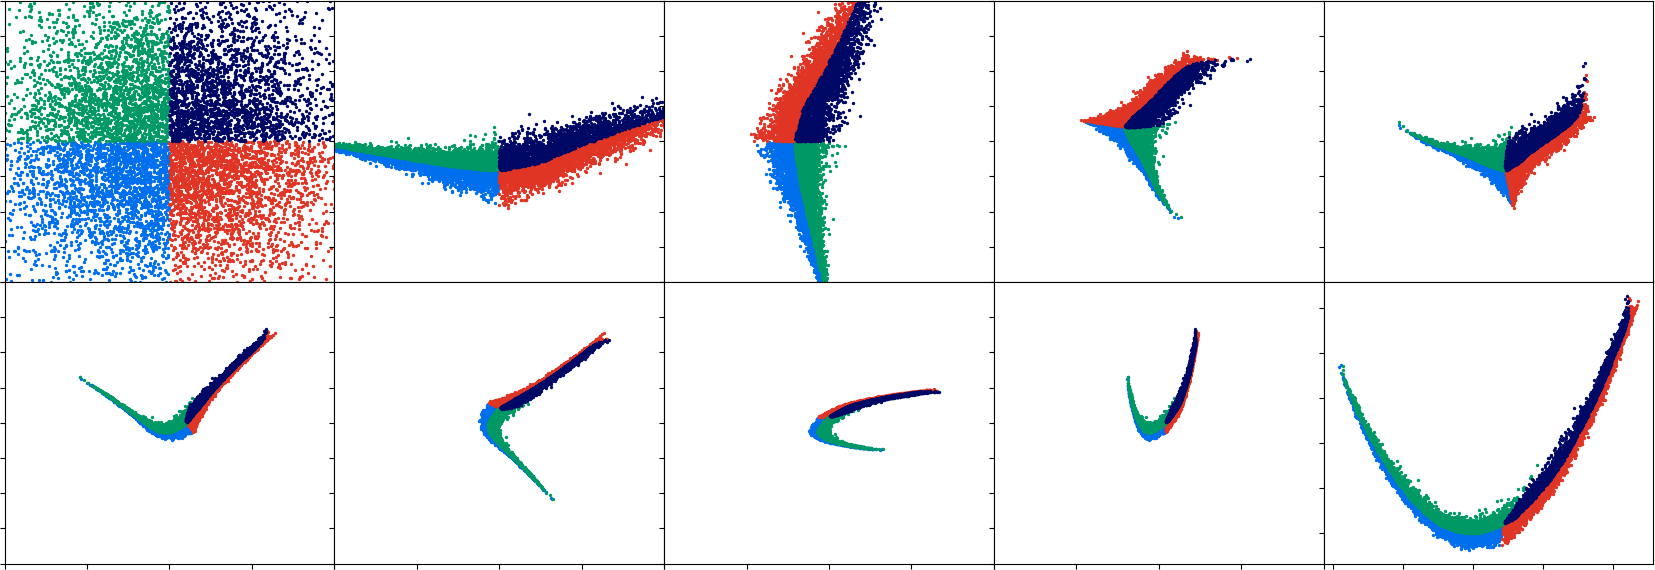
\includegraphics[width=\textwidth]{figures/rosenbrock_flow.png}
                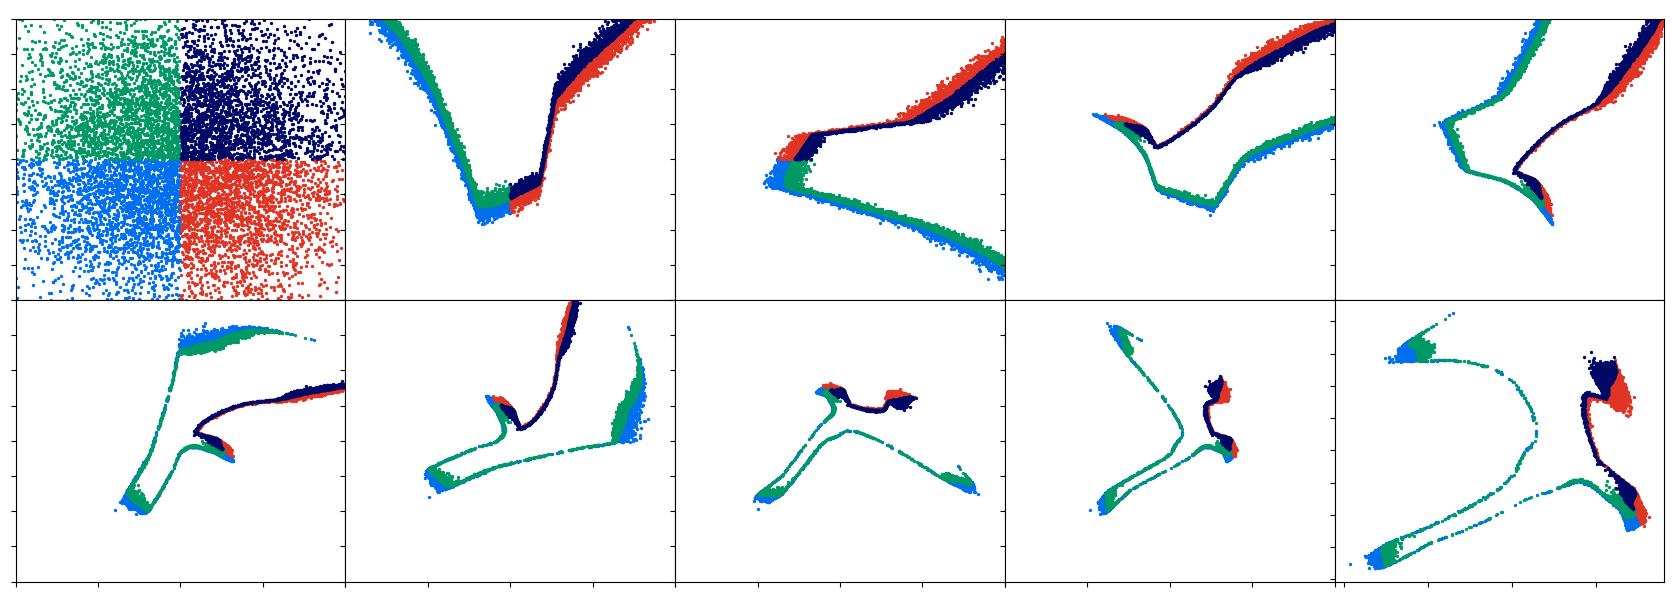
\includegraphics[width=\textwidth]{figures/himmelblau_flow.png}
            }{
                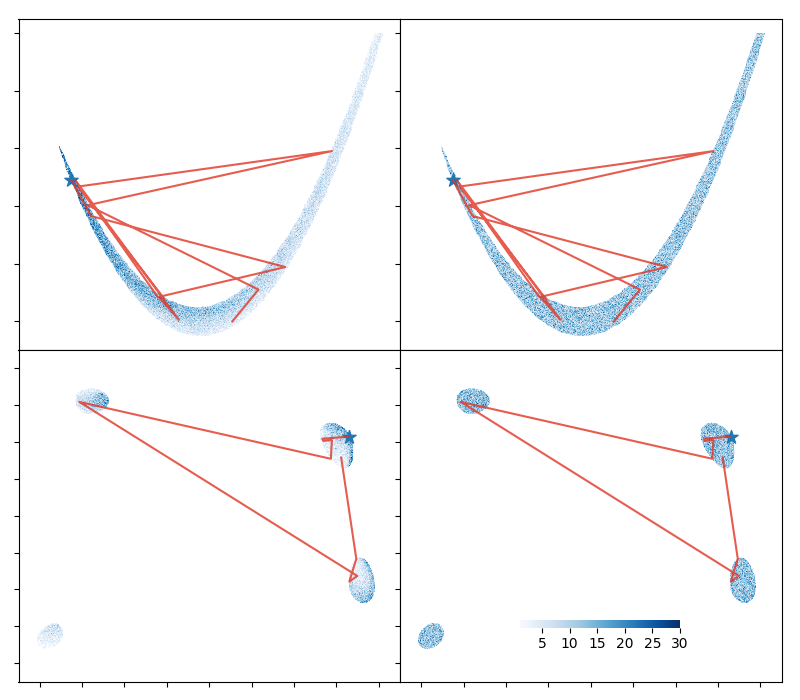
\includegraphics[width=\textwidth]{figures/chains.png}
            }
            \vfill
    }
\end{frame}

\begin{frame}
\end{frame}

\appendix


\begin{frame}
    \frametitle{Key tools for Nested Sampling}
    \begin{description}
        \item[\texttt{anesthetic}] Nested sampling post processing \arxiv{1905.04768}\\
        \item[\texttt{insertion}] cross-checks using order statistics \arxiv{2006.03371}
            \hspace{5pt}\url{github.com/williamjameshandley/anesthetic}
        \item[\texttt{nestcheck}] cross-checks using unthreaded runs \arxiv{1804.06406}\\
            \hspace{5pt}\url{github.com/ejhigson/nestcheck}
        \item[\texttt{MultiNest}] Ellipsoidal rejection sampling \arxiv{0809.3437}\\
            \hspace{5pt}\url{github.com/farhanferoz/MultiNest}
        \item[\texttt{PolyChord}] Python/C++/Fortran state of the art \arxiv{1506.00171}\\
            \hspace{5pt}\url{github.com/PolyChord/PolyChordLite} 
        \item[\texttt{dynesty}] Python re-implementation of several codes \arxiv{1904.02180}\\
            \hspace{5pt}\url{github.com/joshspeagle/dynesty}
    \end{description}
\end{frame}


\begin{frame}
    \frametitle{Nested Sampling: a user's guide}
    \begin{enumerate}
        \item Nested sampling is a likelihood scanner, rather than posterior explorer.
            \begin{itemize}
                \item This means typically most of its time is spent on burn-in rather than posterior sampling
                \item Changing the stopping criterion from $10^{-3}$ to $0.5$ does little to speed up the run, but can make results very unreliable
            \end{itemize}
        \item The number of live points $n_\mathrm{live}$ is a resolution parameter.
            \begin{itemize}
                \item Run time is linear in $n_\mathrm{live}$, posterior and evidence accuracy goes as $\frac{1}{\sqrt{n_\mathrm{live}}}$.
                \item Set low for exploratory runs $\sim\mathcal{O}(10)$ and increased to $\sim\mathcal{O}(1000)$ for production standard.
            \end{itemize}
        \item Most algorithms come with additional reliability parameter(s).
            \begin{itemize}
                \item e.g. \texttt{MultiNest}: $\text{eff}$, \texttt{PolyChord}: $n_\mathrm{repeats}$
                \item These are parameters which have no gain if set too conservatively, but increase the reliability
                \item Check that results do not degrade if you reduce them from defaults, otherwise increase.
            \end{itemize}
    \end{enumerate}
\end{frame}


\end{document}
